\documentclass{standalone}
\usepackage{tikz}
%------------tikz Setup------------

\tikzstyle{ball} = [circle,shading=ball, ball color=black,
    minimum size=1mm,inner sep=1.3pt]
\tikzstyle{miniball} = [circle,shading=ball, ball color=black,
    minimum size=1mm,inner sep=0.5pt]
\tikzstyle{mminiball} = [circle,shading=ball, ball color=black,
    minimum size=0.6mm,inner sep=0.1pt]
\usetikzlibrary{arrows.meta}
\usetikzlibrary{angles, quotes}
\tikzset{>={Latex[length=2mm,width=1.5mm]}}
\tikzset{->-/.style={decoration={markings, mark=at position #1 with
  {\arrow{>}}},postaction={decorate}}}
\usetikzlibrary{decorations.pathmorphing}
\usetikzlibrary{decorations.pathreplacing}
\usetikzlibrary{arrows.meta,calc}
\usetikzlibrary{bending}
\usetikzlibrary{decorations.markings,shapes.geometric}
\tikzset{->-/.style={decoration={markings, mark=at position #1 with
  {\arrow{>}}},postaction={decorate}}}
\tikzset{-|-/.style={decoration={markings, mark=at position #1 with
  {\arrow{stealth}}},postaction={decorate}}}
\tikzset{movearrow/.style 2 args ={
        decoration={markings,
    mark= at position {#1} with {\arrow{#2}} ,
        },
        postaction={decorate}
    }
}


\begin{document}
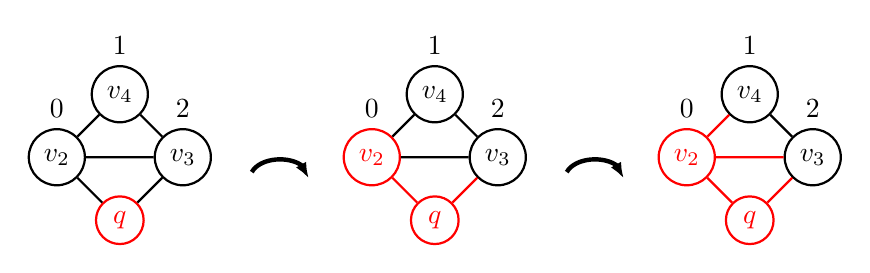
\begin{tikzpicture}[thick,main/.style = {draw, circle}]
\begin{scope}[scale=0.8]
    \node[main,red] (1) at (0,0) {$q$}; 
    \node[main,label={above:$0$}] (2) at (-1,1) {$v_2$};
    \node[main,label={above:$2$}] (3) at (1,1) {$v_3$};
    \node[main,label={above:$1$}] (4) at (0,2) {$v_4$};
    \draw[thick] (1) to (2);
    \draw[thick] (1) to (3);
    \draw[thick] (2) to (4);
    \draw[thick] (3) to (4);
    \draw[thick] (2) to (3);
    \node (a) at (2, 0.6) {};
    \node (b) at (3, 0.5) {};
    \draw[ultra thick,->] (a) to [out=60,in=90] (b);
\end{scope}
\begin{scope}[xshift=4cm,scale=0.8]
    \node[main,red] (1) at (0,0) {$q$}; 
    \node[main,red,label={above:$0$}] (2) at (-1,1) {$v_2$};
    \node[main,label={above:$2$}] (3) at (1,1) {$v_3$};
    \node[main,label={above:$1$}] (4) at (0,2) {$v_4$};
    \draw[thick,red] (1) to (2);
    \draw[thick,red] (1) to (3);
    \draw[thick] (2) to (4);
    \draw[thick] (3) to (4);
    \draw[thick] (2) to (3);
    \node (a) at (2, 0.6) {};
    \node (b) at (3, 0.5) {};
    \draw[ultra thick,->] (a) to [out=60,in=90] (b);
\end{scope}
\begin{scope}[xshift=8cm,scale=0.8]
    \node[main,red] (1) at (0,0) {$q$}; 
    \node[main,red,label={above:$0$}] (2) at (-1,1) {$v_2$};
    \node[main,label={above:$2$}] (3) at (1,1) {$v_3$};
    \node[main,label={above:$1$}] (4) at (0,2) {$v_4$};
    \draw[thick,red] (1) to (2);
    \draw[thick,red] (1) to (3);
    \draw[thick,red] (2) to (4);
    \draw[thick] (3) to (4);
    \draw[thick,red] (2) to (3);
\end{scope}
\end{tikzpicture}
\end{document}